
\documentclass[tikz, border=10pt]{standalone}
\usetikzlibrary{arrows}

\def\h{1.5cm}
\def\w{4.2cm}
\def\m{0.1cm}
\def\lw{0.3mm}

\begin{document}
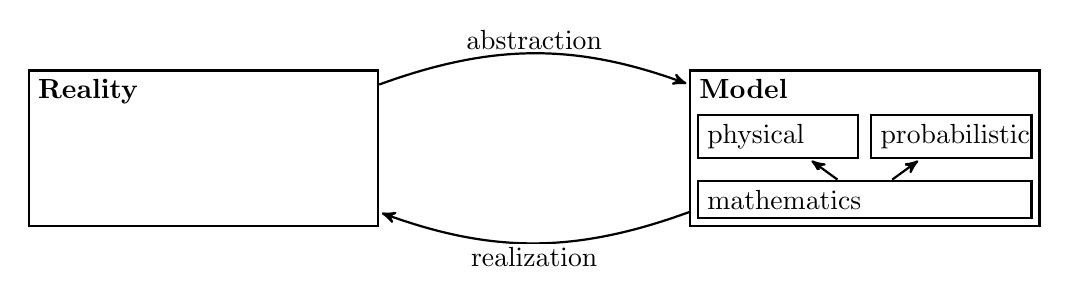
\begin{tikzpicture}[->,>=stealth',shorten >=1pt,auto,
		thick]

  \node[line width=\lw, draw, text depth=\h , text width=\w ,font=\normalsize] at (-2*\w, 0) 	(R){\textbf{Reality}};
  
  \node[line width=\lw, draw, text depth=\h , text width=\w, font=\normalsize] at (0,0) (M){\textbf{Model}};
  \node[draw, text width=\w/2-3*\m] at (-\w/4-\m/2,\h/10) (Phy) {physical};
  \node[draw, text width=\w/2-3*\m] at (\w/4+\m/2,\h/10) (Pr) {probabilistic};
  \node[draw, text width=\w-2*\m] at (0,-\h/2+\m) (Math) {mathematics};

  \path[every node/.style={font=\normalsize,
  		fill=white,inner sep=1pt}]
  	% Right-hand-side arrows rendered from top to bottom to
  	% achieve proper rendering of labels over arrows.
    (R) edge [bend left=20] node {abstraction} (M)
    
    (Math) edge [bend left=0] node {} (Phy)
    (Math) edge [bend left=0] node {} (Pr)
        
  	% Left-hand-side arrows rendered from bottom to top to
  	% achieve proper rendering of labels over arrows.
    (M) edge [bend left=20] node {realization} (R);
    
\end{tikzpicture}
\end{document}